%% This is file `DEMO-TUDaPub.tex' version 2.09 (2020/03/13),
%% it is part of
%% TUDa-CI -- Corporate Design for TU Darmstadt
%% ----------------------------------------------------------------------------
%%
%%  Copyright (C) 2018--2020 by Marei Peischl <marei@peitex.de>
%%
%% ============================================================================
%% This work may be distributed and/or modified under the
%% conditions of the LaTeX Project Public License, either version 1.3c
%% of this license or (at your option) any later version.
%% The latest version of this license is in
%% http://www.latex-project.org/lppl.txt
%% and version 1.3c or later is part of all distributions of LaTeX
%% version 2008/05/04 or later.
%%
%% This work has the LPPL maintenance status `maintained'.
%%
%% The Current Maintainers of this work are
%%   Marei Peischl <tuda-ci@peitex.de>
%%   Markus Lazanowski <latex@ce.tu-darmstadt.de>
%%
%% The development respository can be found at
%% https://github.com/tudace/tuda_latex_templates
%% Please use the issue tracker for feedback!
%%
%% ============================================================================
%%
% !TeX program = lualatex
%%

\documentclass[
	ngerman,
	accentcolor=1c,% Farbe für Hervorhebungen auf Basis der Deklarationen in den Corporate Design Richtlinien
%	logofile=example-image, %Falls die Logo Dateien nicht vorliegen
	]{tudapub}

\usepackage[english, main=ngerman]{babel}
\usepackage[babel]{csquotes}

\usepackage{biblatex}
\bibliography{DEMO-TUDaBibliography}

%Formatierungen für Beispiele in diesem Dokument. Im Allgemeinen nicht notwendig!
\let\file\texttt
\let\code\texttt
\let\pck\textsf
\let\cls\textsf

\usepackage{hologo}




\begin{document}

%Zusätzliche Metadaten für PDF/A. In diesem Fall notwendig, weil Titel ein Makro enthält.
\Metadata{
	author=NeXT,
	title=Space Workshop Rating,
	%subject=Basisdokumentation und Template zur Nutzung der tudapub-Dokumentenkasse,
	%date=2019-04-29,
	%keywords=TU Darmstadt \sep Corporate Design \sep LaTeX
}




\title{Lego EV3\newline Lejos-Einrichtung}
\subtitle{NeXT Generation on Campus}
%\author{Marei Peischl\thanks{pei\TeX{} \TeX{}nical Solutions}\and der \TeX-Löwe}
\date{}
%\titleimage{
%%	%Folgende Box kann selbstverständlich durch ein mit \includegraphics geladenes Bild ersetzt werden.
%\bigskip
%\bigskip
%\bigskip
%\bigskip
%\bigskip
%\bigskip
%\bigskip
%\bigskip
%\bigskip
%\bigskip
%\bigskip
%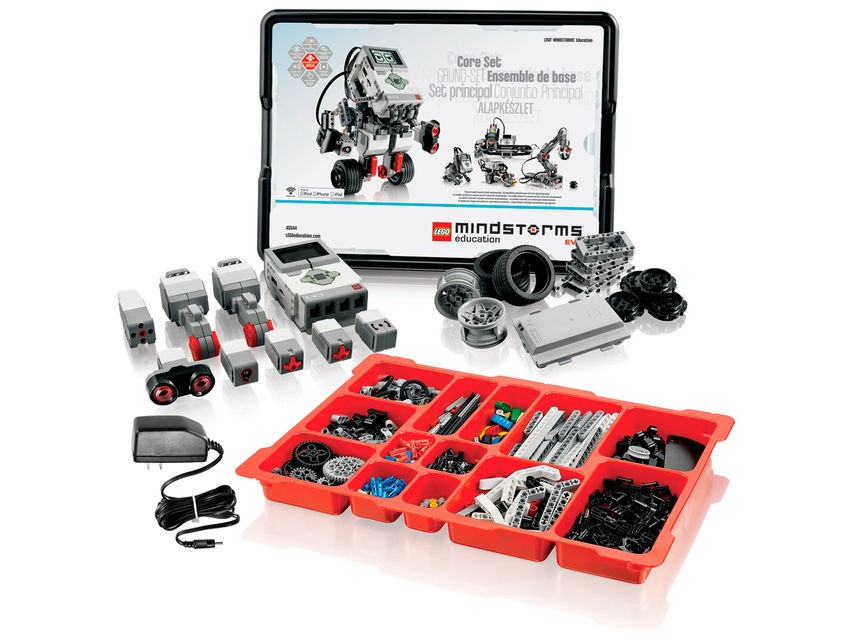
\includegraphics[width=\textwidth]{../control/images/title.jpg}
%	%\color{black!30}\rule{\width}{\height}
%}


%Varianten der Infoboxen
\addTitleBox{\includegraphics[width=\linewidth]{../../ist_logo.pdf}}
%\addTitleBoxLogo{example-image}
%\addTitleBoxLogo*{\includegraphics[width=.3\linewidth]{example-image}}



\maketitle


\newpage


\tableofcontents

\section{Einf\"uhrung}
F\"ur die verschiedenen Workshops ist verschieden viel Material notwendig. Als Beispiele sind die von uns erfolgreich genutzten Hardware-Komponenten gelistet, mit anderen Ger\"aten sollte die Software ebenso laufen.\newline
Im Abschnitt \ref{Space-Workshop} wird beschrieben, welche Hardware f\"ur den grundlegenden Aufbau ben\"otigt wird, w\"ahrend f\"ur den Mindroid-Workshop noch die Komponenten aus Abschnitt \ref{Space-Workshop} verwendet werden.\newline
Im Abschnitt \ref{git-repos} wird auf das von uns genutzte Material eingegangen.\\
Abschnitt \ref{EinrichtungPC} beschreibt die grundlegende Einrichtung des PCs \"ur den Space-Workshop und Abschnitt \ref{Einrichtung-Mindroid} die ben\"otigten Vorbereitungen f\"ur den Mindroid-Workshop.
\subsection{Space-Workshop}
\label{Space-Workshop}
\begin{description}
	\item[PC]
	\item[EV3]
	\item[microSD] m\"oglichst maximal 8GB
\end{description}

\subsection{Mindroid-Workshop}
\label{Mindroid-Workshop}


\begin{description}
	\item[WLAN-Dongle] z.B. Edimax EW-7811Un
	\item[Smartphone] z.B. Google Nexus 5
	\item[Router] z.B. 
\end{description}

\subsection{Ben\"otigte Git-Repositories}
\label{git-repos}
Um den Space-Workshop durchzuf\"uhren sind keine weiteren Dateien von uns notwendig, sie dienen aber als Unterst\"utzung f\"ur den Beginn. F\"ur den Mindroid-Workshop ist mindestens das repository mit dem Quellcode zwingend notwendig.\newline
In diesem
\href{https://github.com/NeXT-Workshops/NeXT-Instructions}{\textbf{repository}\footnote{$https://github.com/NeXT-Workshops/NeXT-Instructions$}}
befinden sich für den Space-Workshop eine Dokumentation mit den wichtigsten Befehlen sowie eine m\"ogliche Punktewertung des Szenarios, sowie eine Dokumentation und m\"ogliche Aufgaben und L\"osungen f\"ur den Mindroid-Workshop.
\href{https://github.com/NeXT-Workshops/NeXT-Projects}{\textbf{Hier}\footnote{$https://github.com/NeXT-Workshops/NeXT-Projects$}}
befinden sich APIs zur Vereinfachung der Bearbeitung, das bedeutet, dass mit verschiedenen Niveaustufen, unterschiedlich viele Hilfestellungen gegeben werden. Diese k\"onnen einfach heruntergeladen werden und entsprechend in intelliJ ge\"offnet werden.


\section{Einrichtung der PCs- Grundlagen}
\label{EinrichtungPC}
Im Folgenden werden die verschiedenen Schritte für die Einrichtung der PCs erl\"autert. Diese Anleitung gilt ausschlie\ss{}lich f\"ur Windows-PCs. Eine Einrichtung unter Linux und MACOS ist jedoch ebenfalls m\"oglich.\newline
Der Link f\"uhrt direkt zum Download, sodass die Installation entsprechend der weiteren Anweisungen durchgef\"uhrt werden kann.\newline

\subsection{Java Developement Kit}
Um den Programmcode f\"ur den Roboter zu schreiben, ist ein JDK notwendig, welches, falls noch nicht vorhanden, 
\href{https://download.oracle.com/otn/java/jdk/8u231-b11/5b13a193868b4bf28bcb45c792fce896/jdk-8u231-windows-x64.exe}{\textbf{hier}\footnote{$https://download.oracle.com/otn/java/jdk/8u231-b11/5b13a193868b4bf28bcb45c792fce896/jdk-8u231-windows-x64.exe$}}
mit einem kostenlosen Oracle-Konto heruntergeladen werden kann. Falls sich auf dem PC ein \"alteres 32-Bit Betriebssystem befindet ist 
\href{https://download.oracle.com/otn/java/jdk/8u231-b11/5b13a193868b4bf28bcb45c792fce896/jdk-8u231-windows-i586.exe}{\textbf{dieser Link}\footnote{$https://download.oracle.com/otn/java/jdk/8u231-b11/5b13a193868b4bf28bcb45c792fce896/jdk-8u231-windows-i586.exe$}}
richtig.\newline
Damit die folgenden Programme Java finden, m\"ussen die Systemvariablen gesetzt werden. Zu Diesen gelangt man \"uber \textit{Systemsteuerung} \rightarrow{} \textit{System und Sicherheit} \rightarrow{} \textit{System} \rightarrow{} \textit{erweiterte Systemeinstellungen}. Dort gibt es das Feld \textit{Umgebungsvariablen}, mit dem man zu einem Fenster mit den \textit{Systemvariablen} gelangt. Dort muss der Path mit \textit{Bearbeiten} erg\"anzt werden. Im Feld \textit{Wert der Variablen} muss folgender Befehl hinzugef\"ugt werden:\newline
F\"ur 64-Bit-Systeme:\\$;C:\backslash ProgramFiles\backslash Java\backslash jdk1.8.0\_231\backslash bin$\newline
F\"ur 32-Bit-Systeme:\\$;C:\backslash ProgramFiles(x86)\backslash Java\backslash jdk1.8.0\_231\backslash bin$\\
Als N\"achstes wird \textit{JAVA\_HOME} gesetzt. Unter \textit{Systemvariablen} wird mit \textit{Neu} ein \"ahnliches Fenster ge\"offnet, bei dem als  \textit{Name der Variable JAVA\_HOME} und als Wert Folgendes gesetzt wird:\newline
F\"ur 64-Bit-Systeme:\\$C:\backslash ProgramFiles\backslash Java\backslash jdk1.8.0\_231$\newline
F\"ur 32-Bit-Systeme:\\$C:\backslash ProgramFiles(x86)\backslash Java\backslash jdk1.8.0\_231$\\
\subsection{LeJOS}
Als N\"achstes folgt die Installation von leJOS, die Schnittstelle zwischen dem PC und dem Roboter. Das Programm kann
\href{https://sourceforge.net/projects/ev3.lejos.p/files/0.9.1-beta/leJOS\_EV3\_0.9.1-beta\_win32\_setup.exe/download}{\textbf{hier}\footnote{$https://sourceforge.net/projects/ev3.lejos.p/files/0.9.1-beta/leJOS\_EV3\_0.9.1-beta\_win32\_setup.exe/download$}}
heruntergeladen werden und entsprechend der Anweisungen installiert werden.\newline
Falls ein anderes Betriebssystem genutzt wird, befinden sich
\href{https://sourceforge.net/projects/ev3.lejos.p/files/0.9.1-beta/}{\textbf{hier}\footnote{$https://sourceforge.net/projects/ev3.lejos.p/files/0.9.1-beta/$}} weitere Versionen und entsprechende Installationsanweisungen.

\subsection{Ejre}
Damit der Roboter den Java-Code verarbeiten kann, muss ein neues Betriebssystem auf der MicroSD-Karte installiert werden. Daf\"ur wird das ejre8 empfohlen, auch
\href{https://www.oracle.com/java/technologies/javaseembedded7u75-downloads.html}{\textbf{ejre ARMv5}\footnote{$https://www.oracle.com/java/technologies/javaseembedded7u75-downloads.html$}}
ist m\"oglich. In unseren Workshops verwenden wir ejre 8, welches aber nicht offiziell von oracle zur Ver
\href{https://download.oracle.com/otn/java/jdk/8u231-b11/5b13a193868b4bf28bcb45c792fce896/jdk-8u231-windows-i586.exe}{\textbf{ejdk}\footnote{$https://download.oracle.com/otn/java/jdk/8u231-b11/5b13a193868b4bf28bcb45c792fce896/jdk-8u231-windows-i586.exe$}} ben\"otigt.

\subsection{IntelliJ}
Zur Programmierung wird eine IDE ben\"otigt, wir verwenden dazu in unseren Workshops intelliJ, welche 
\href{https://download.jetbrains.com/idea/ideaIC-2018.3.6.exe?_ga=2.13038195.579836862.1576405054-449566094.1572879017}{\textbf{hier}\footnote{$https://download.jetbrains.com/idea/ideaIC-2018.3.6.exe?_ga=2.13038195.579836862.1576405054-449566094.1572879017$}}
heruntergeladen werden und entsprechend der weiteren Anweisungen installiert werden kann. Zur Kommunikation mit dem Roboter muss ein entsprechendes Plugin installiert werden, dies möglicht über \textit{Datei} \rightarrow{} \textit{Einstellungen} \rightarrow{} \textit{Plugins}. Danach findet man das entsprechende Plugin mit dem Suchbegriff \textit{ev3}, sodass man es \"uber \textit{installieren} dem Programm hinzuf\"ugen kann.

\section{Einrichtung der Roboter}
Um dieses Betriebssystem auf dem Roboter zu installieren, muss das Programm unter \textit{$C:\backslash Program Files\backslash leJOS EV3\backslash bin$} gestartet werden. Bei einem anderen Installationsort \"andert sich entsprechend auch dieser Pfad.\newline
Danach muss die eingesteckte microSD-Karte als Laufwerk ausgew\"ahlt werden und das soeben heruntergeladene EJRE ausgew\"ahlt werden. Mit \textit{Create} wird dann die Software auf der microSD-Karte installiert und kann in den Roboter gesteckt werden um sie mit einem Start des Roboters zu installieren.

\section{Einrichtung Mindroid}
\label{Einrichtung-Mindroid}
Dieser Abschnitt ist nur relevant, wenn der Mindroid-Workshop durchgef\"uhrt werden soll.

\subsection{PC}
F\"ur die Kommunikation zum Handy m\"ussen auf dem PC verschiedene Regeln in der Firewall hinzugef\"ugt werden. Zum Einen muss das verwendete JDK die Erlaubnis bekommen, über das Netzwerk kommunizieren zu dürfen. Zum anderen müssen je nach Konfiguration der Firewall noch Regeln hinzugefügt werden, dass über die Ports 5555 und 33044 mit UDP und TCP empfangen und gesendet werden darf.

\subsection{Handy}
Damit auf den Handys die Mindroid-App installiert werden kann, dazu m\"ussen die Handys gerootet werden, dazu gibt es im Internet verschiedene Anleitungen für das entsprechende Modell. Wir verwenden in unseren Workshops \href{https://lineageos.org/}{\textbf{LineageOS}\footnote{$https://lineageos.org/$}}.
\subsection{Router}

\subsection{Roboter}
Auf dem Roboter muss f\"ur die Nutzung ein spezielles Programm gestartet werden, welches vorher \"uber das Skript \textit{script} \"ubertragen werden kann.

\section{Pr\"asentation}
Unter folgendem \href{https://www.dropbox.com/sh/9ffsq69el4c4kf4/AADeHAn5SQX5iI4gcCer6Ll_a?dl=0}{\textbf{Link}\footnote{$https://www.dropbox.com/sh/9ffsq69el4c4kf4/AADeHAn5SQX5iI4gcCer6Ll_a?dl=0$}} 
sind die von uns genutzten Pr\"asentationen zu finden, hierbei ist es aber immer sinnvoll, den Inhalt an das Niveau und Alter der Zuh\"orer anzupassen. Hierbei k\"onnen in angepasstem Umfang Hilfestellungen zur Programmiersprache gegeben werden.\newline
MindroidIntro ist eine Pr\"asentation f\"ur den Workshop inklusive Handys, w\"ahrend MindroidSmall f\"ur die Version ohne Handys mit Kabel\"ubertragung ist. Space beinhaltet dementsprechend ein\"uhrende Folien f\"ur den Space-Workshop. In der Mindroid-Challenge-Pr\"asentation befindet sich ein m\"oglicher Vorschlag f\"ur einen Wettkampf im Rahmen des Mindroid-Workshops.

%\end{figure}


\cfoot{\textcolor{lightgray} \today}




\end{document}
